%\documentclass[12pt,a4paper]{book}
\documentclass[12pt,a4paper]{report}

\usepackage{xeCJK}
\usepackage{makeidx}

%楷体
\setCJKmainfont{AR PL UKai CN}

% 将日期变为中文格式
\renewcommand{\today}{\number\year 年 \number\month 月 \number\day 日}

\makeindex
\printindex
\setcounter{secnumdepth}{5}

\title{路由器反向供电商业计划书}
\author{微度无限}

\begin{document}
\maketitle
\tableofcontents

%最多三级标题
%\chapter{章}
%\section{节}
%\subsection{子节}

%%本命令用于重新定义摘要标题为中文"摘要"
\renewcommand{\abstractname}{摘\quad 要}
\begin{abstract}
宽带运营商的机房设备(交换机等)供电均来自与小区供电系统。受小区物业管理、电费等因素影响,运营商在机房投入高昂。本项目可以大幅度减小运营商的机房成本。
\end{abstract}

\chapter{团队介绍}
待施工……

\chapter{需求及解决方案}
目前宽带运营商机房供电基本采取独立供电方案,本项目提供改造方案和新品两个方案,下面结合图\ref{供电}分析现有供电的问题和我们解决的问题。
\begin{enumerate}
    \item 传统供电,从机房取电,受制于小区物业管理,并且按照商业用电计费,运营成本高昂。
    \item 改造方案,从用户路由取点,不受小区物业限制,并且按照居民用电计费,运营成本低廉。但是相较于传统的供电方式,改造后系统变复杂,需要一定的改造成本。
    \item 新品方案,解决了改造方案的系统变复杂的缺点,但是对于已经联网的小区实施有一些困难。
\end{enumerate}
结合三种方案的优缺点,对于已联网的小区实施改造,新建小区实施新品方案较合适。
\begin{figure}
    \begin{center}
    %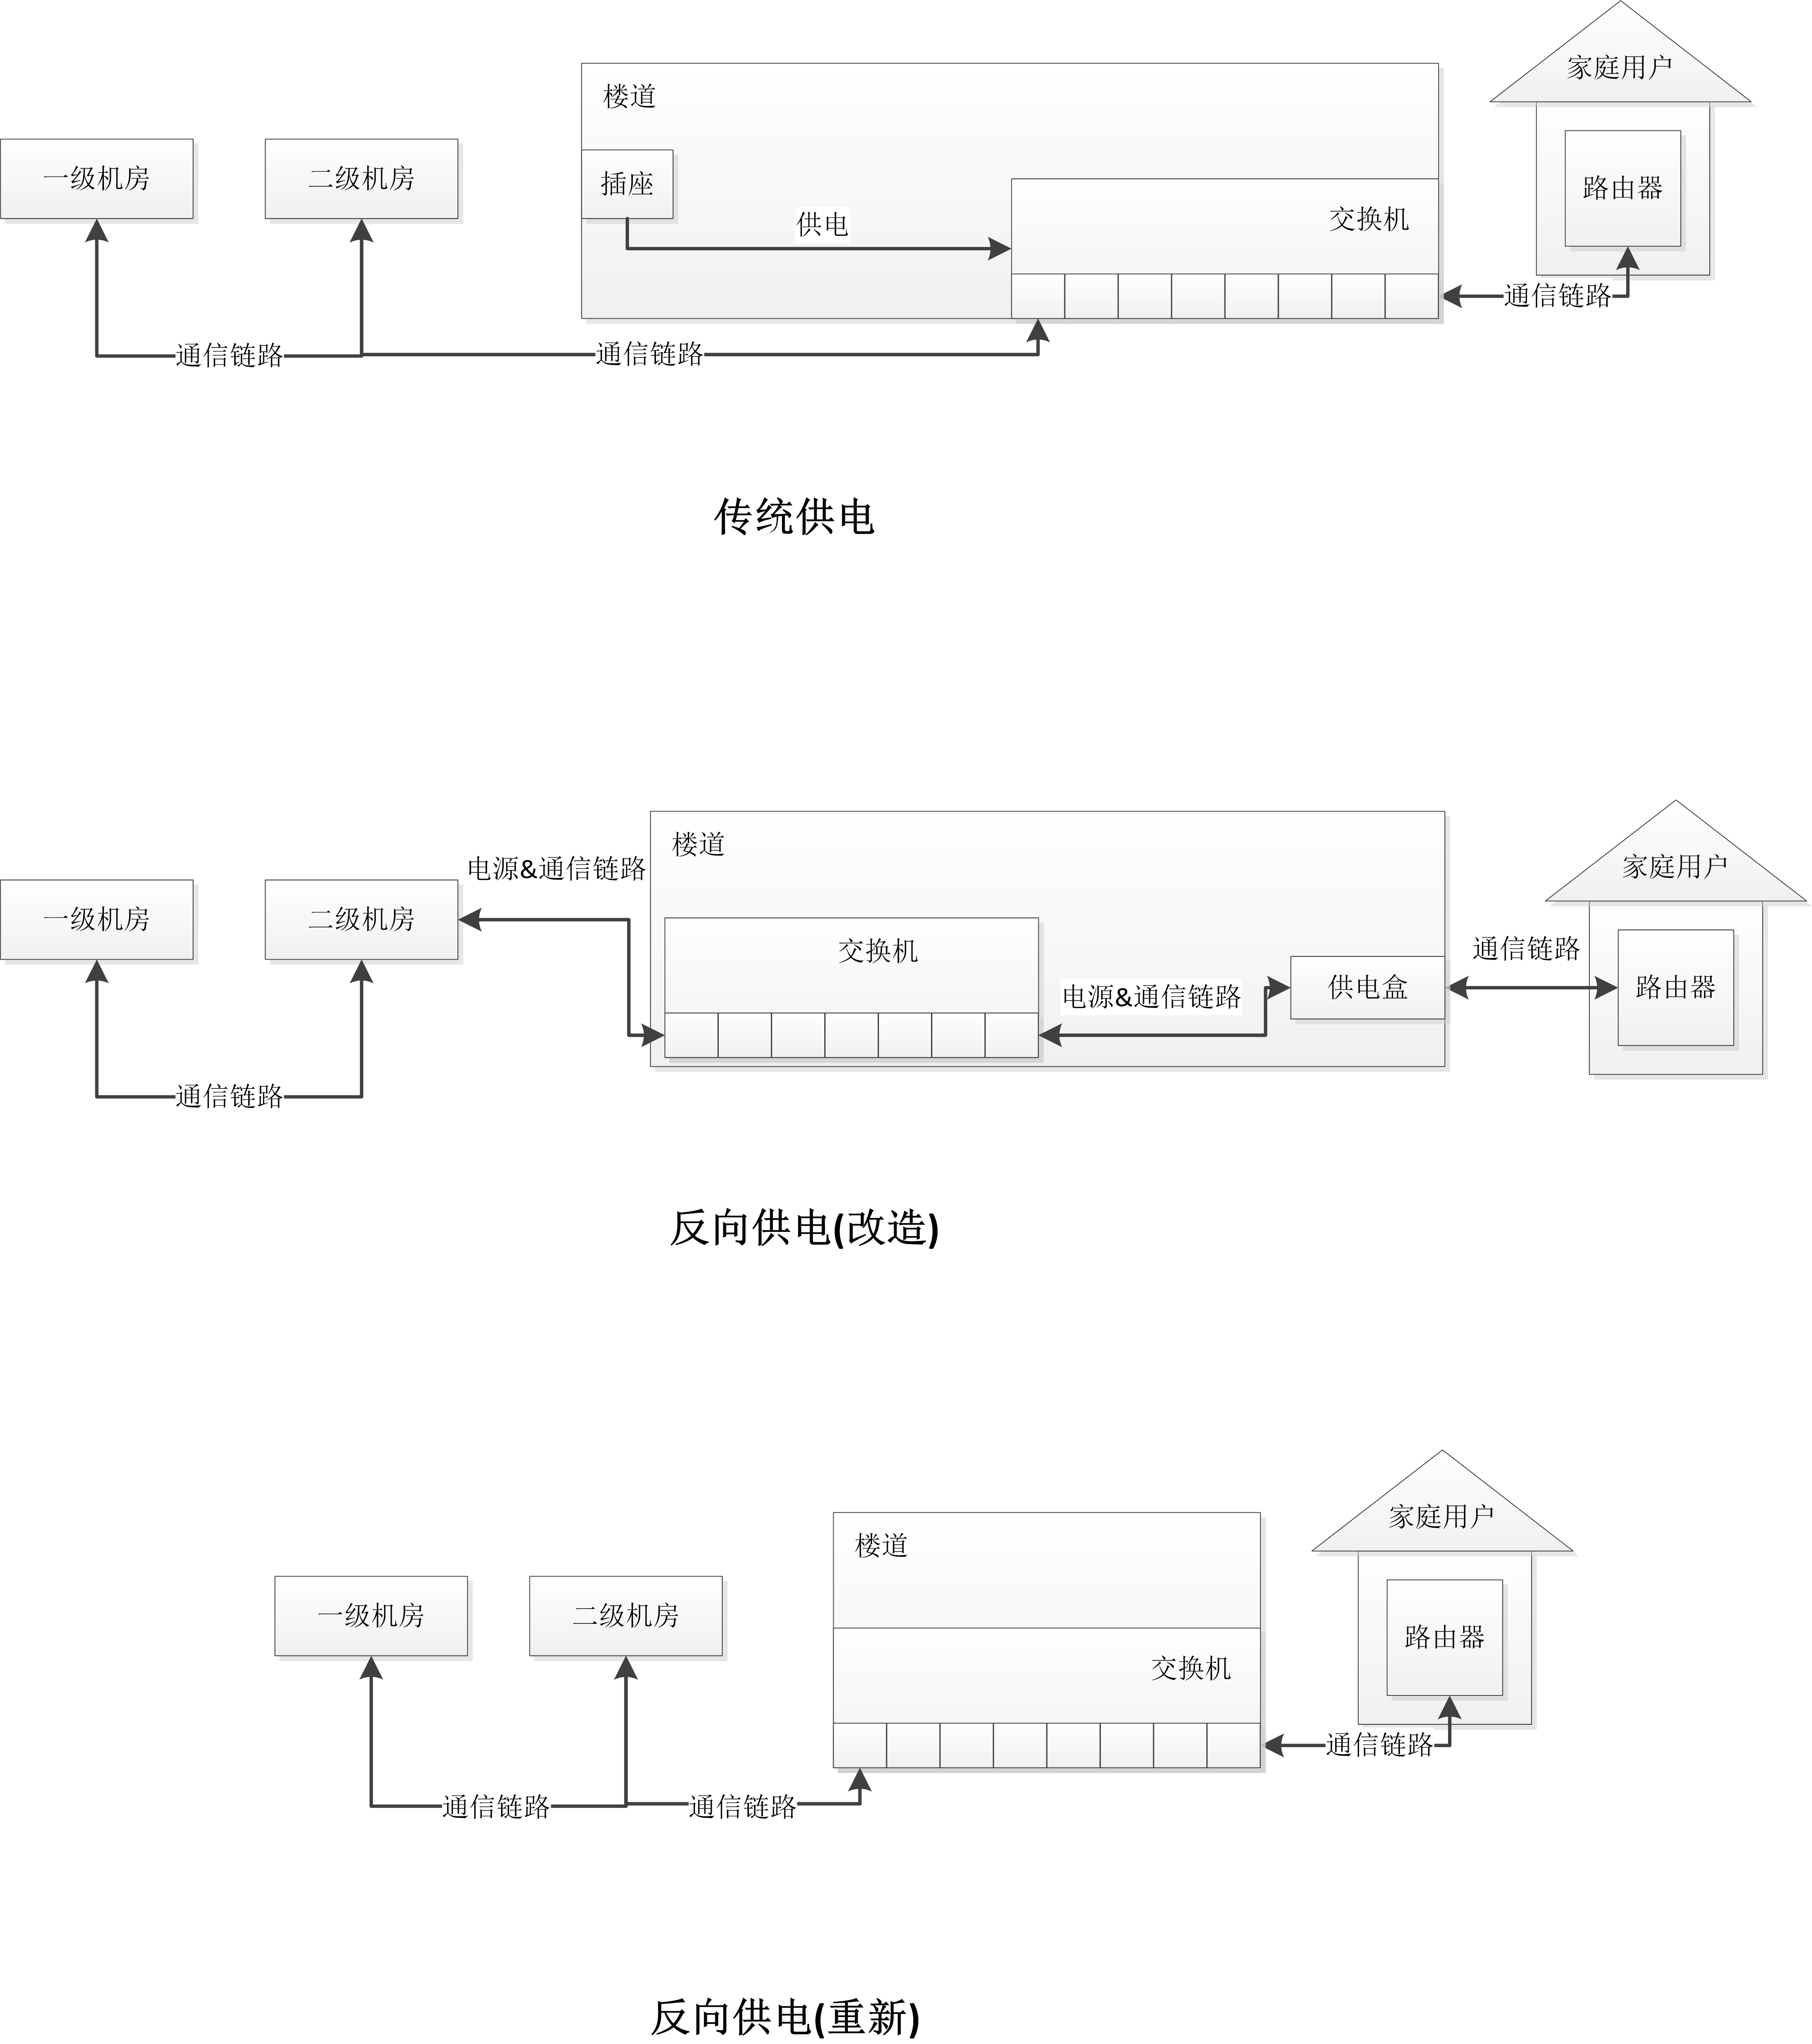
\includegraphics[width=0.5\textwidth]{fig/供电.jpg}
    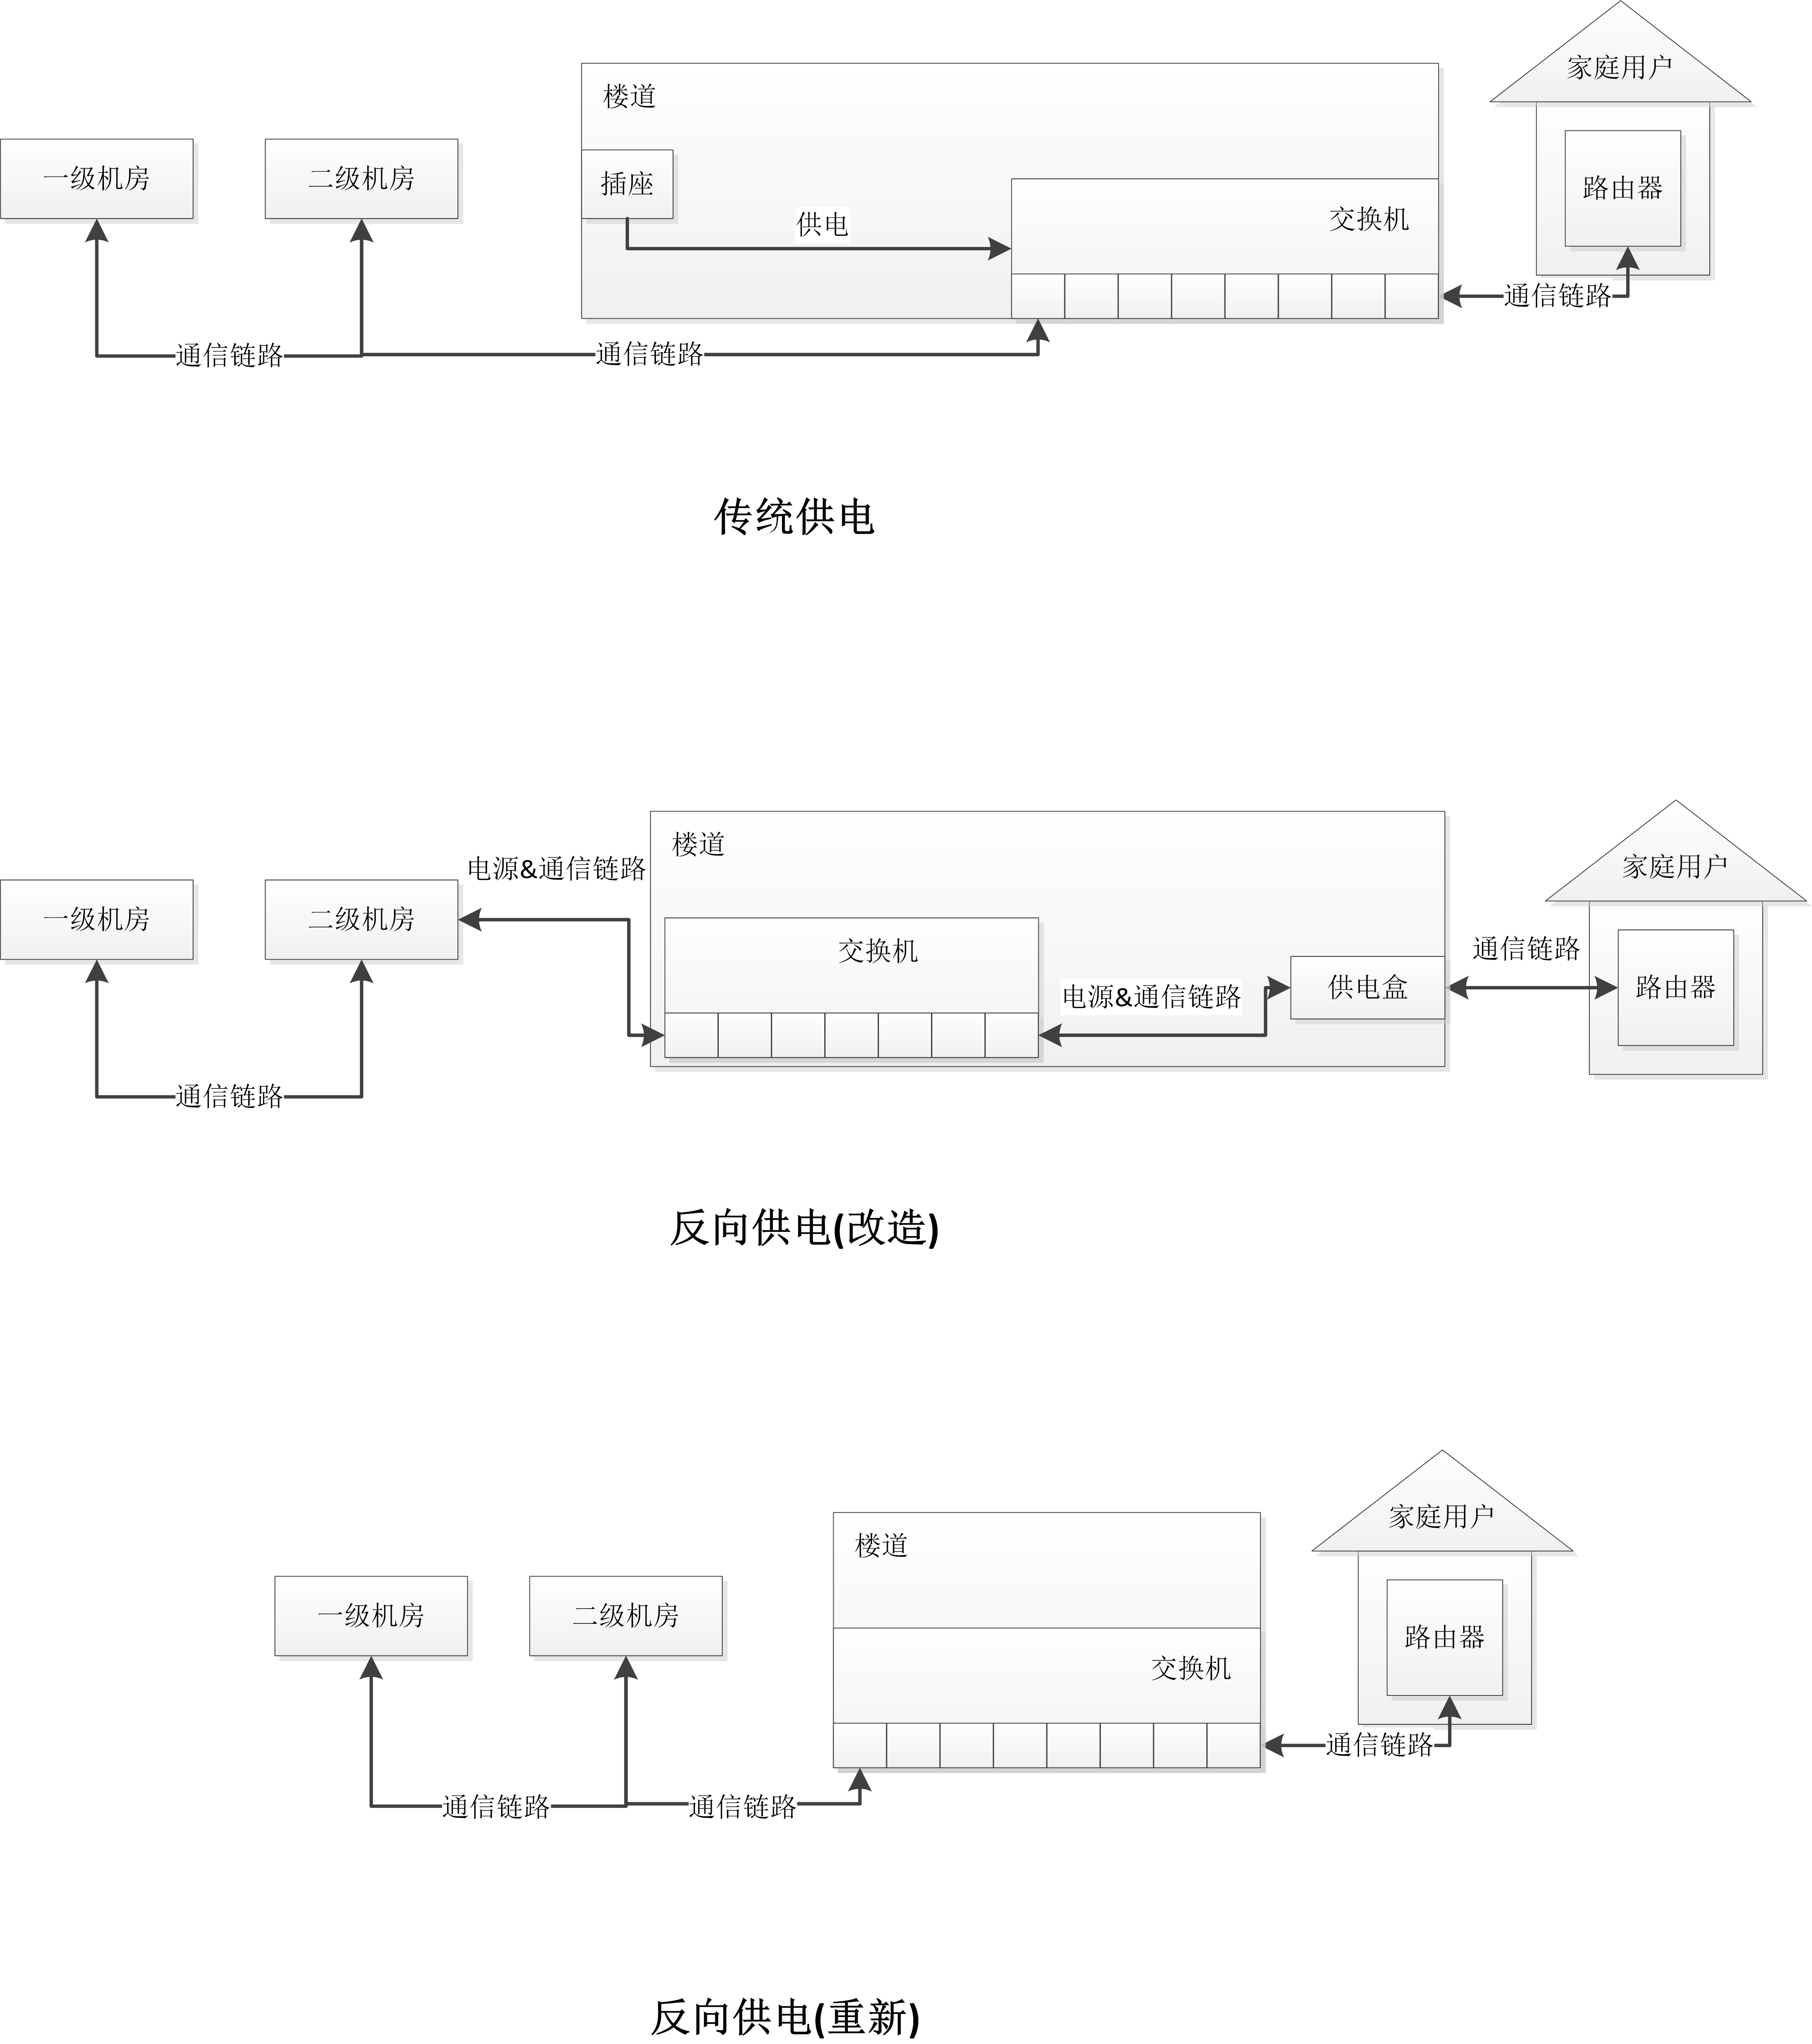
\includegraphics[width=0.9\textwidth]{fig/供电.jpg}
    \caption{供电方案}
    \label{供电}
    \end{center}
\end{figure}

\chapter{市场分析}
本章结合路由器反向供电方案,首先计算单台交换机的改造成本,然后分析其产生的效益,最后分析全球市场容量。
\section{成本}
采用路由器反向供电方案后,需要对现有路由器、交换机进行改造,改造成本是一次性投入。每台交换机的改造成本为:
\begin{equation}
    cost = cC + nPort \times cRP + cCP
    \label{成本}
\end{equation}
其中各变量的含义如表\ref{成本公式变量}
\begin{table}[!hbp]
    \begin{center}
        \begin{tabular}{|l|l|l|}
            \hline
            变量名 & 涵义 & 值(元) \\
            \hline
            cC & 供电转换盒成本 & 60 \\
            \hline
            nPort & 交换机端口数 & 16 \\
            \hline
            cRP & 路由器供电安全保护本 & 10 \\
            \hline
            cCP & 供电转换盒子安全保护成本 & 10 \\
            \hline
            cost & 单台交换机改造成本 & 150 \\
            \hline
        \end{tabular}
        \caption{成本公式变量\label{成本公式变量}}
    \end{center}
\end{table}
由公式\ref{成本}可以计算出单台交换机样品改造成本为150元人民币,批量生产后成本有望下降1/3,即100元/台以内。
\section{效益}
采用独立电源供电方案,运营商的成本有两个方面构成:
\begin{enumerate}
    \item 派遣人员与物业沟通的费用
    \item 电费
\end{enumerate}
保守计算将第一项费用忽略,这里只计算电费。首先给出独立供电的电费计算公式\ref{独立供电电费}:
\begin{equation}
    costOrig = pS * 24 * 365 * pB
    \label{独立供电电费}
\end{equation}
然后同理可得路由器反向供电电费\ref{路由器反向供电电费}:
\begin{equation}
    costNow = pS * 24 * 365 * pR
    \label{路由器反向供电电费}
\end{equation}
路由器反向供电的效益为独立供电成本减去路由器反向供电成本,得出效益公式\ref{效益}:
\begin{equation}
    benefit = pS * 24 * 365 * (pB - pR)
    \label{效益}
\end{equation}
公式\ref{独立供电电费}公式\ref{路由器反向供电电费}公式\ref{效益}中各变量的含义如表\ref{效益变量}
\begin{table}[!hbp]
    \begin{center}
        \begin{tabular}{|l|l|l|}
            \hline
            变量名 & 涵义 & 值 \\
            \hline
            costOrig & 独立供电成本(元/年) & 124.83 \\
            \hline
            costNow & 反向供电成本(元/年) & 75.29 \\
            \hline
            pS & 交换机功率(W) & 15 \\
            \hline
            pB & 商业电价(元/度) & 0.95 \\
            \hline
            pR & 居民电价(元/度) & 0.573 \\
            \hline
            benefit & 单台效益(元/年) &  49.54 \\
            \hline
        \end{tabular}
        \caption{效益变量\label{效益变量}}
    \end{center}
\end{table}
将表\ref{效益变量}中的值带入公式\ref{效益}:中可以得到单台交换机采用路由器反向供电后每年的效益为49.54元/年,结合之前的改造成本100元/台,故可以得出大概两年就可以收回改造成本的结论。
\section{市场容量}
据宽带论坛(BroadbandForum)最新发布的报告称,2013年全球宽带增长达到了新高,而中国的宽带用户数则位列全球第一位。Broadband Forum的报告显示,去年全球宽带的增长达到了过去5年来的新高,其中全球宽带用户增长6549.36万,宽带用户总数达到了5.97亿,年增长率达到12.3\%。另外,在各个国家和地区中,中国宽带用户数达到1.58亿,位列全球第一,年增长率为20.35\%。根据经验数据,交换机和家用路由器的比例为1:10,故交换机的数量约为用户数的1/10。
由以上报告可以得出:
\begin{enumerate}
    \item 全球市场容量约为:30亿/年
    \item 中国的市场容量为:7.5亿/年
    \item 全球新增效益:3亿/年
    \item 中国新增效益:1亿/年。
\end{enumerate}

\chapter{竞争性分析}
待施工……

\end{document}

